\documentclass{article}
\usepackage[utf8]{inputenc}
\usepackage[spanish]{babel}
\usepackage{listings}
\usepackage{graphicx}
\graphicspath{ {images/} }
\usepackage{cite}

\renewcommand{\familydefault}{\sfdefault}

\begin{document}

\begin{titlepage}
    \begin{center}
        \vspace*{1cm}
            
        \Huge
        \textbf{Parcial 1}
            
        \vspace{0.5cm}
        \LARGE
            
        \vspace{5cm}
            
        \textbf{Juan David Martinez Bonilla}\\
        \textbf{Emmanuel Garay Rivera}\\
        \textbf{Sofia Marin Cacante}
            
        \vfill
            
        \vspace{0.8cm}
            
        \Large
        Departamento de Ingeniería Electrónica y Telecomunicaciones\\
        Universidad de Antioquia\\
        Medellín\\
        Abril de 2021
            
    \end{center}
\end{titlepage}

\tableofcontents

\newpage
\section{\large Problemas para resolver }\\\\
A continuación se irán enumerando y documentando por fecha los problemas que van surgiendo al resolver el examen parcial con su respectivo análisis y solución/decisión tomada.\\

\subsection{\large Problema 1.}\\\\	Organización y disposición de los componentes electrónicos (19/04/21).\\

\textbf{\large Análisis}\\\\
Para tener un control organizado de la matriz 8x8 de leds se plantea la idea de usar dos circuitos integrados 74HC595 \cite{johann}, uno para conectar los ánodos de las luces leds y otro para conectar los cátodos de dichas luces.
La intención de esto es tener un sistema de referencia por “coordenadas” que permita ubicar cada led requerido de forma fácil y rapida.\\

\textbf{\large Implementación}\\
\begin{figure}[h]
    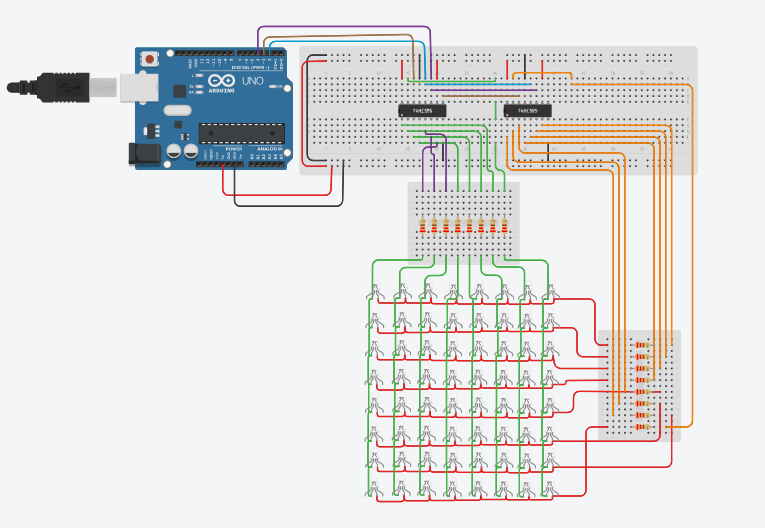
\includegraphics[width=8cm]{Imagen1.png}
    \centering
    \caption{Primer circuito}
    \label{fig:Imagen1}
\end{figure}\\\\

\subsection{\large Problema 2.}\\\\
Conectando los componentes de la forma planteada en la solucion del problema 1 se detectó que, al prender todos los leds (de forma "manual") se quemaban los circuitos integrados, no permitían un óptimo desarrollo del programa y se presentaban inconvenientes a la hora de realizar algunos patrones básicos (20/04/21).\\


\textbf{\large Solución}\\\\
Se rediseñó el circuito de tal manera que al seguir las compuertas lógicas de la siguiente tabla de verdad, los circuitos integrados no se quemaban, además de permitir (siguiendo la misma tabla de verdad) un diseño de algoritmo más eficiente y con posibilidad de ingresar cualquier patrón sin problema.\\

\begin{figure}[h]
    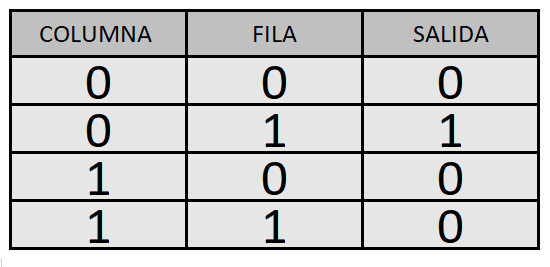
\includegraphics[width=8cm]{Tabla de verdad.png}
    \centering
    \caption{Tabla de verdad}
    \label{fig:Tabla de verdad}
\end{figure}\\\\

\begin{figure}[h]
    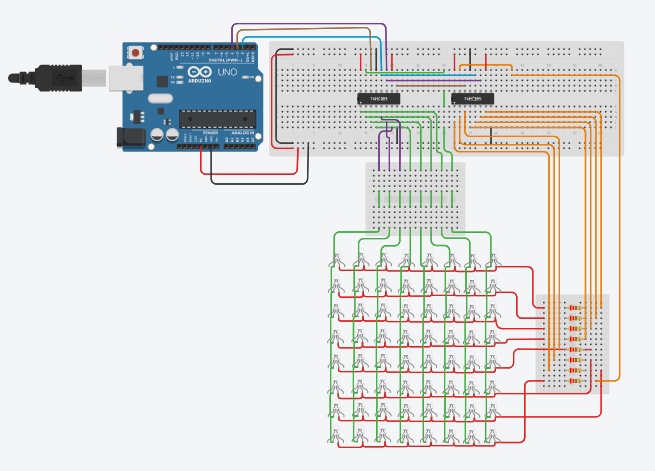
\includegraphics[width=8cm]{Imagen2.png}
    \centering
    \caption{Segundo circuito}
    \label{fig:Imagen2}
\end{figure}\\\\

\subsection{\large Problema 3.}\\\\
¿Como recibir los patrones que el usuario quiera ingresar y traducir cada parte del patrón a la posición del led correspondiente? (19/04/21).\\
\\\\\
\\

\textbf{\large Análisis}\\\\
Como idea principal se plantea nombrar e identificar cada posición de la matriz de leds, de forma que mediante una grafica mostrada en el manual de uso, el usuario pueda identificar que leds desea prender mediante el numero propio de cada led, además con el orden establecido de los números se puede dar la opción al usuario de prender varios leds al tiempo mediante un rango ingresado entre el 1 y el 64.
\\
\\
Ejemplo:
\\
\\
1\  \ 2\ \ \ 3\  \ 4\ \ \ 5\  \ 6\ \ \ 7\  \ 8\\ 
- \  \  - \  \ - \  \ - \  \ - \  \ - \  \ - \   \ -\\
- \  \  - \  \ - \  \ - \  \ - \  \ - \  \ - \   \ -\\
- \  \  - \  \ - \  \ - \  \ - \  \ - \  \ - \   \ -\\
- \  \  - \  \ - \  \ - \  \ - \  \ - \  \ - \   \ -\\
- \  \  - \  \ - \  \ - \  \ - \  \ - \  \ - \   \ -\\
- \  \  - \  \ - \  \ - \  \ - \  \ - \  \ - \   \ -\\
57 58 59 60 61 62 63 64\\

\textbf{\large Implementación}\\\\
\begin{figure}[h]
    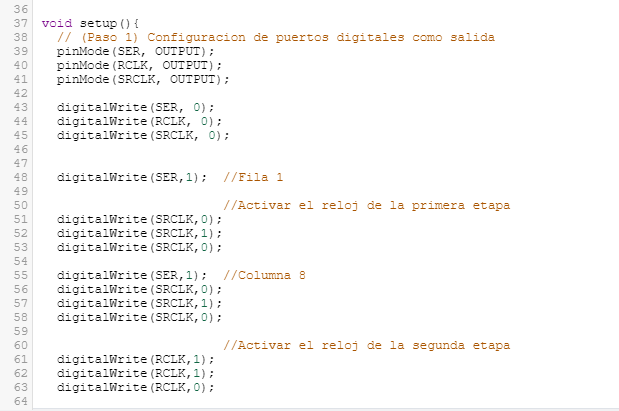
\includegraphics[width=8cm]{Imagen3.png}
    \centering
    \caption{Primer codigo}
    \label{fig:Imagen3}
\end{figure}\\\\

Después de inicializar las variables del pin de entrada (SER), reloj de desplazamiento (SRCLK) y reloj de registro de salida (RCLK), en modo OUTPUT, se realizó el desplazamiento de cada dato de forma manual, para analizar el funcionamiento e ir interiorizándolo, permitiendo crear patrones básicos.\\

\subsection{\large Problema 4.}\\\\
Al intentar realizar el desarrollo del problema 3 se concluyó que dicho método tenía poca optimización para implementar el programa al hacerlo de forma “manual” , además se detectaron problemas al querer desarrollar patrones complejos, dado que el sistema de filas y columnas anteriormente implementado, generaba un conflicto cuando se deseaba prender algunos patrones intermitentes (su forma no era continua/lineal) (21/04/21). \\

\textbf{\large Solución}\\\\
1. Se descartó la idea de enumerar cada posición de la matriz de muestra (del 1 al 64) junto con la idea de permitir que el usuario ingrese un rango de valores para encender ese número de leds siguiendo el orden numérico descartado anteriormente.\\\\
2. Se recurrió al uso de la función shiftOut \cite{arduino} la cual recibe 4 parámetros:\\

-dataPin\\

-clockPin\\

-bitOrder\\

-value\\
\\\\

Permitiéndonos así configurar la matriz de una forma más ordenada y sencilla, además de que con el método de entrada por bits (siguiendo la tabla de verdad  de la figura 2) e implementando el método de desplazamiento por barrido \cite{veritasium} se puede lograr una ilusión de imagen solida logrando imprimir cualquier patrón sin ningún inconveniente.\\\\
\\\\
\\\\
\\\\
\\

\textbf{\large Implementación}\\
\begin{figure}[h]
    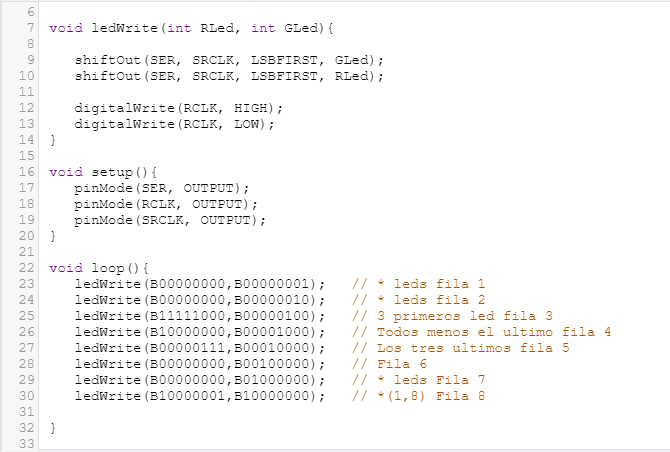
\includegraphics[width=8cm]{Imagen4.png}
    \centering
    \caption{Segundo codigo}
    \label{fig:Imagen4}
\end{figure}
\begin{figure}[h]
    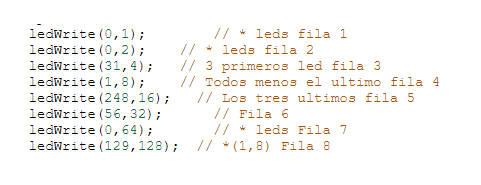
\includegraphics[width=10cm]{Imagen5.png}
    \centering
    \caption{Segundo codigo (forma 2)}
    \label{fig:Imagen4}
\end{figure}\\\\
\\\\
\subsection{\large Problema 5.}\\\\
Después de imprimir cualquier patrón se llegó a la conclusión de que los tiempos de ejecución eran infinitos, nunca terminaban, por esto surgió la necesidad de ejecutar ciclos en T tiempo (21/04/21). \\

\textbf{\large Solución}\\\\
después de analizar diferentes opciones como delay, o librerías como time.h se decidió implementar millis, ya que este sigue su conteo mientras van ejecutando los ciclos.
Basándose del código extraído de \textbf{ArduWiki} \cite{arduwiki}.\\\\

\textbf{\large Implementación}\\\\
\begin{figure}[h]
    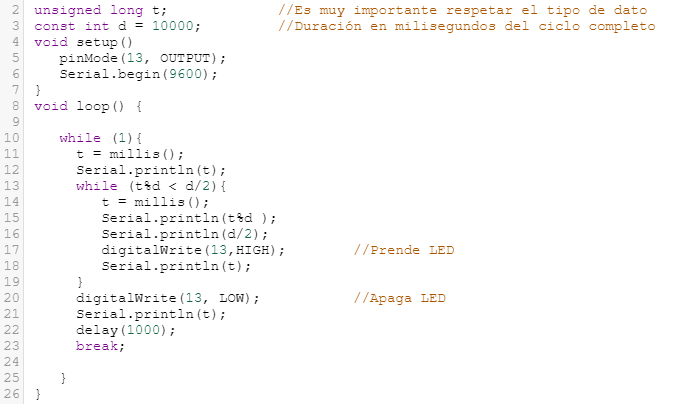
\includegraphics[width=8cm]{Imagen6.png}
    \centering
    \caption{Tercer codigo}
    \label{fig:Imagen6}
\end{figure}\\\\


\section{\large Diseño de funciones}\\\\
\subsection{\large Funcion verificación (full)}\\\\
Esta función crea una matriz bidimensional cuyo contenido está en memoria dinámica, creando una columna de ceros y otra columna dependiente de la posición de la fila.\\
Ejemplo:\\\\
(0,1) == (B00000000,B00000001)\\
(0,2) == (B00000000,B00000010) \\
(0,4) == (B00000000,B00000100) \\ 
(0,8) == (B00000000,B00001000) \\
(0,16) == (B00000000,B00010000) \\
(0,32) == (B00000000,B00100000) \\
(0;64) == (B00000000,B01000000) \\
(0,128) == (B00000000,B10000000) \\
\\
\textbf{\large Codigo}\\\\
\begin{figure}[h]
    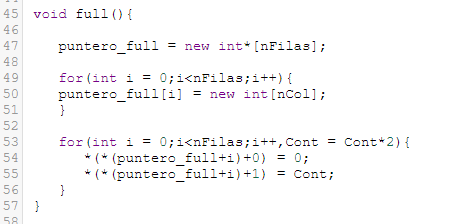
\includegraphics[width=8cm]{Imagen7.png}
    \centering
    \caption{Cuarto codigo}
    \label{fig:Imagen7}
\end{figure}\\\\
\subsection{\large Funcion clear}\\\\
Se basa en la función verificación, con una modificación: en lugar de colocar un cero en la columna uno, coloca un 255, limpiando así toda la matriz.\\\\
(255,1) == (B11111111,B00000001)\\
(255,2) == (B11111111,B00000010) \\
(255,4) == (B11111111,B00000100) \\ 
(255,8) == (B11111111,B00001000) \\
(255,16) == (B11111111,B00010000) \\
(255,32) == (B11111111,B00100000) \\
(255;64) == (B11111111,B01000000) \\
(255,128) == (B11111111,B10000000) \\
\\
\textbf{\large Codigo}\\\\
\begin{figure}[h]
    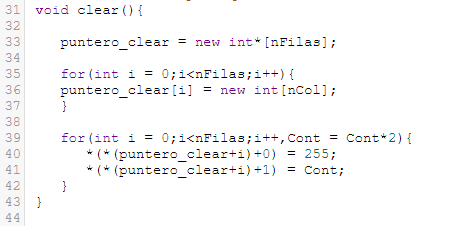
\includegraphics[width=6cm]{Imagen8.png}
    \centering
    \caption{Quinto codigo}
    \label{fig:Imagen8}
\end{figure}\\\\
\subsection{\large ledWrite}\\\\
Esta función recibe como argumentos dos enteros (int) bien sea en notación binaria o decimal (0-255).
Esta función se usa en conjunto con la función shiftOut, primero se envían los datos de la segunda posición de los argumentos ya que como se sabe los datos se van desplazando al enviarlos de forma serial. para finalizar se realiza un flanco de subida en el reloj de registro de salida.\\
\\
\textbf{\large Codigo}\\\\
\begin{figure}[h]
    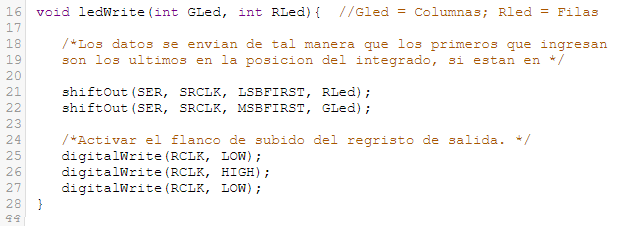
\includegraphics[width=8cm]{Imagen9.png}
    \centering
    \caption{Sexto codigo}
    \label{fig:Imagen9}
\end{figure}\\\\

\subsection{\large print-Matriz}\\\\
Imprime una matriz 2x8\\\\

\textbf{\large Codigo}\\\\
\begin{figure}[h]
    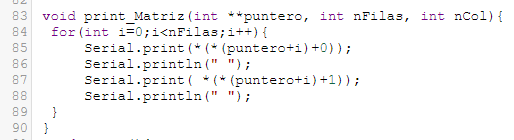
\includegraphics[width=8cm]{Imagen11.png}
    \centering
    \caption{Septimo codigo}
    \label{fig:Imagen9}
\end{figure}\\\\

\subsection{\large image}\\\\
\\
Le permite al usuario mostrar un patrón en la matriz de leds.\\

\textbf{\large Codigo}\\\\
\begin{figure}[h]
    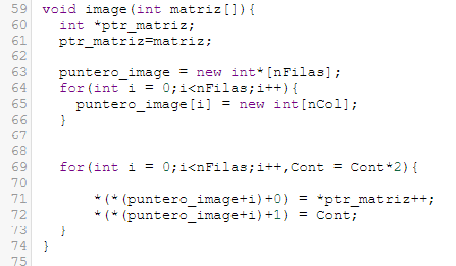
\includegraphics[width=8cm]{Imagen10.png}
    \centering
    \caption{Octavo codigo}
    \label{fig:Imagen9}
\end{figure}\\\\


\newpage

\bibliographystyle{IEEEtran}
\bibliography{references}

\end{document}